\documentclass[../main/thesis_msc.tex]{subfiles}

\begin{document}

\chapter{Imaging}
In this thesis, we have imaged two galaxies- IC 342 and NGC 628, using the HBA data.\\

\section{NGC 628}
NGC628 is an almost face-on grand design late-type spiral galaxy. It is located at a distance of almost 7.3~Mpc \citep{ngc_distance}. Details on the galaxy can by found in the Table \ref{ngc_intro}. It has two clearly defined spiral arms that can be seen in any optical image of the galaxy. In the UV, the spiral arms can be seen as bright knots on diffuse emission \citep{2001ApJS..132..129M}, and these knots are also tracd in the H$\alpha$. It is an isolated galaxy, and does not have strong density waves. HI holes have been detected in the HI layer of the galaxy, with sizes ranging from 0.24~kpc to 2~kpc \citep{2011AJ....141...23B}. The galaxy is seen to consist of two disks, the inner disk being 8-10~kpc. These regions span different type of stellar populations \citep{1992A&A...256...79N}, with a colder inner region \citep{2006MNRAS.367...46G}, and faint H II regions covering the outer part of the galaxy \citep{1538-3881-116-2-673}. The H I distribution is seen to be extended and asymmetric to the southwest. In \citep{1992A&A...253..335K}, it was seen that the inner part of the galaxy has a flat differentially rotating disk while the outer part is not a ``well-behaved" disk. In \citep{2003ApJS..146..353M} it was concluded that the inner part of the galaxy has no dust lanes, while outer part of the galaxy has clear nuclear dust spirals.

\begin{table}[h]
        \centering
        \begin{tabular}{cc}
        \hline\hline
            Distance\footnote{\citep{ngc_distance}} & $\sim$7.3~Mpc\\
            Position\footnote{\citep{nobody_cares}} & RA:01h36m41.74s\\ 
                     & DEC:+15d47m01.1s\\
            
            Morphology\footnote{\citep{morphology}} & SA(s)c\\
            Star Formation Rate\footnote{\citep{2008AJ....136.2648D}} & 1.21~M$_\odot$/year\\
            Inclination angle- inner disk (deg)\footnote{\citep{1992A&A...253..335K}} & 7\\
            Inclination angle- outer disk (deg) \footnote{\citep{1992A&A...253..335K}} & 13.5\\
            Position angle (deg) \footnote{\citep{1992A&A...253..335K}} & 02 \\
             \hline
        \end{tabular}
        \caption{Parameters of NGC628}
        \label{ngc_intro}
    \end{table}

\section{IC 342}
IC 342 is an intermediate, almost face-on spiral galaxy of the Maffei 1/IC 342 group, the galaxy group nearest to our Local group, at a distance of around 3.3~Mpc\citep{distance_ic342}. Details on the galaxy can by found in the Table \ref{ic342_intro}. There has been a great amount of interest in the study of the galaxy, as it has a structure most similar to our own galaxy with similar dynamical mass (2 $\times$ 10$^8$ M$_\odot$) \citep{dyn_mas}. The super massive black hole mass at the center of IC 342 is also of the same order ($\sim 10^6$~M$_\odot$) as Milky Way. It is only 10.6$~\deg$ above the galactic plane, and is not clearly visible because of the Galactic disk and the large number of foreground stars in optical regime. It is the third largest spiral galaxy in the sky, with an angular size of . It consists of a central nuclear star cluster, where a lot of the star formation occurs. There exist five prominent Giant Molecular Clouds (GMCs) in the molecular ring and the arms, each of the mass of approximately 10$^6$ M$_{\odot}$ \citep{ic342_2}. The nucleus of the galaxy consists of two mini-spiral arms that are connected to the inner molecular ring. This structure is seen due to the presence of barred potential, which is also indicated by the morphology of the velocity residuals\footnote{Subtracting the the rotation model with the observed velocities gives the residual velocities} which showed the presence of a large bipolar structure \citep{H1}. The outer part of the galaxy can be seen to have four distinct arms, with the inner part having speeds up to 38 $\pm$ 7~km s$^{-1}$kpc$^{-1}$ and the outer part ($\sim$ 5~kpc frm center) having a speed of around 11 $\pm$ 6~km s$^{-1}$kpc$^{-1}$ \citep{arms}. Photodissociation Region (PDR) is present within the central 400~pc of IC 342 \citep{ic342_1}. The physical and chemical geometry can be best understood from diagram \ref{swr} of IC 342. The yellow regions represent the H II regions. The star formation in the nuclear region was studied using Radio Recombination Lines (RRLs) and continuum emission at C- band and Ka-band with the JVLA, and two components were resolved lying east and west of the central star cluster, which were associated with two GMCs. It was predicted that several compact H II regions provide best fit for the two regions \citep{ic342_3}. It is at a low inclination of 31 $\deg$, according to the HI kinematic data, which also indicates the counter-clockwise rotation of the galaxy \citep{H1}. With the help of H II and S II filters, 16 Supernova Remnants were identified, most of them being near or in the H II regions and two of them isolated \citep{snr}. IC 342 is also the host of four Ultra Luminous X-ray sources (ULX) \citep{ulx}. 

\begin{table}[t]
        \centering
        \begin{tabular}{cc}
            \hline\hline
            Position\footnote{\citep{ic342_position}} & RA:03h46m48.503s\\ 
                     & DEC:+68d05m46.92s\\
            Distance\footnote{\citep{distance_ic342}} & $\sim$3.3~Mpc\\
            Morphology\footnote{\citep{morphology}} & SAB(rs)cd\\
            Star Formation Rate\footnote{\citep{SFR}} & 2.8~M$_\odot$/year\\
            Inclination angle (deg)\footnote{\citep{H1}} & 30 \\
            Position angle (deg)\footnote{\citep{H1}} & 39.4 \\
            B$_T$ (mag)\footnote{\citep{nobody_cares}} & 9.16 \\
             \bottomrule
        \end{tabular}
        \caption{Parameters of IC 342}
        \label{ic342_intro}
    \end{table}
\begin{figure}[h]
\centering
\includegraphics[scale = 0.25]{turner_IC342}
\caption{Schematic of the chemical and physical structure of the nucleus of IC 342\citep{ic342_4}}
\label{swr}
\end{figure}

Being an axis symmetric spiral (ASS), over the years, magnetic fields in this galaxy have been studied at several wavelengths- 6.2 and 11~cm \citep{grave}, at 20~cm \citep{ic342_20}. Recently, Faraday tomography of the local ISM with LOFAR, in \citep{ic342_5}, showed the presence of two Faraday thin neutral clouds clearly separated in Faraday depth.  In this thesis, we have also studied the polarized sources in the field of view of the galaxy at frequencies as low as 150~MHz. More information about the magnetic fields in IC 342 can be found in section \ref{magnetic}.

\section{Observational setup}
\textbf{NGC628:} The observations for NGC 628 were done in an interleaved mode. The calibrator used was 3C 48, and the scans were alternatively taken from the target to the calibrator. The observation used 14 remote stations and 23 core stations. The number of stations used for the observation of NGC 628 was 37. No international stations were used. Details of the observation can be found in the table \ref{setup}. The baselines used for the observation can be seen in figure \ref{baseline} that shows the uv distance in meters and amplitude plot. 
\begin{table}[h]
        \centering
        \begin{tabular}{cc}
            \hline\hline
            Start date (UTC) & 22-Nov-2013 / 15:19:00.0 \\ 
            End date (UTC) & 23-Nov-2013 / 00:50:59.9\\
            Interleaved calibrator & 3C48\\
            Scan length on calibator & 2~min\\
            Scan length on target & 20~min\\
            Duration of observation & 9~hours 32~min\\
            Final time on target & 8~hours (24 scans)\\
            Frequency range (from Pre-factor) & 110.667-179.027~MHz\\
            Frequency range (for Factor) & 110.667-169.239~MHz\\
            Total bandwidth on target & 68.36~MHz\\
            Final bandwidth in target & 58.57~MHz\\
             \hline
        \end{tabular}
        \caption{Parameters of NGC628}
        \label{setup}
    \end{table}

\begin{figure}[h]
	%\centering
	\subfloat[]{{\includegraphics[scale=0.2]{uvdist.png}}}
	\centering
	\subfloat[]{{\includegraphics[scale=0.2]{zoom.png}}}
	\caption{This was the arrangement of baselines used for the observation. This is a plot generated by task in CASA called 'plotms' for the first measurement set for the frequency 111~MHz in the first time step. From the plot, one can see the baselines used in terms of meters. As can be seen, the observation uses a dense core to image diffuse flux in the galaxy- the disk and the halo parts. \textit{Right:} This image shows the shorter baselines used. The shortest projected baseline used was around 23~m. }
	\label{faceting}
	\end{figure}

%\begin{figure}[h]
%\centering
%\includegraphics[scale = 0.25]{uvdist.png}
%\caption{This was the arrangement of baselines used for the observation. This is a plot generated by task in CASA called 'plotms' for the first measurement set for the frequency 111~MHz in the first time step. From the plot, one can see the baslines used in terms of meters. As can be seen, the observation uses a dense core to image diffuse flux in the galaxy- the disk and the halo parts.}
%\end{figure}

\newpage
\section{Calibration of LOFAR data}
Calibration in LOFAR is especially difficult due to the ionosphere that causes delay differences between antenna stations. This gives rise to additional phase errors in the visibilities that vary station to station due to LOFAR's large array size. This phase depends on two factors: (1) Free electron column density along the line of sight, (2) Frequency being observed. Another aspect to be noted while calibration of LOFAR is the station beam shape that varies with time and also, the difference between the beam model and the actual beam shape.\\
Inorder to take care of these effects, LOFAR data calibration involves two major parts. In this thesis, a tool called Factor\footnote{\url{https://github.com/lofar-astron/factor}} was used. The major steps to the data reduction are explained below. An overview on how to use the tool itself is described in a later section \ref{overview_factor}.

\subsection{Direction independant part}

The first step to do direction independant calibration is the flagging of RFI (Radio Frequency Interference) with the help of \href{https://sourceforge.net/projects/aoflagger/}{AOFlagger} \citep{aoflagger}. Then, the data is averaged using \href{https://www.astron.nl/lofarwiki/doku.php?id=public:user_software:documentation:ndppp}{NDPPP} to be 4s in time resolution and 4 channels per subband in frequency resolution, to reduce the size of the data. Then, all baselines with CS013 HBA station were flagged and a flux density scale was created for 3C 48 (which was chosen as the amplitude calibrator source) using the model that shows the flux density values of the source at several different frequencies, with a flux density of 64.76~Jy at 150~MHz. Using this primary beam calibrator, the gain solutions are obtained using \verb|BlackBoard Selfcal| (BBS) for all four correlations. The gain solutions are then transferred to the target\citep{BBS} data to correct for the instrumental effects\footnote{\textbf{Instrumental effects:}  The clocks at the remote stations are not perfectly synchronized, which causes a phase delay. This in addition to the phase delay by the ionosphere gives rise to phase errors. The phase difference for a baselines can be written as: \begin{center}
$\Delta$ phase($\nu$,t) =  $\underbrace{ \vphantom{\frac{8.448 \times 10^9 \textrm{p}_1 \textrm{(t)}}{\nu}} 2\pi \textrm{p}_0\textrm{(t)} \nu}_{\textbf{Clock difference effects}}$ - $\underbrace{\frac{8.448 \times 10^9 \textrm{p}_1 \textrm{(t)}}{\nu}}_{\textbf{Total Electron Content (TES) effects}}$ [rad] \end{center} Here $\nu$ represents frequency and p$_0$ and p$_1$ represents the clock difference and TEC difference. These errors need to be removed. This is done with the help of a bright source with a high Signal to Noise ratio on all baselines. Brute force search is done to obtain clock and TEC initial guesses, as computing using the equation is not computationally feasible.}. The A team sources affect the visibilities through the side lobes of the station beam. Hence, the visibilities in which the contribution is more than 5~Jy (in apparent flux density) [ask Rainer] are flagged. This was followed by another round of flagging, and averaging. The data was concatenated into subbands with time resolution of 8~s. The width of each channel was kept at 48.828~kHz, and the total bandwidth was at 1.95~MHz. The last step in direction independant calibration involves the subtraction of soures by first subtracting clean components in medium resolution images, and then reimaging the subtracted image at a lower resolution (1.5' and uv cut range of 2~k$\lambda$) and full field of view image [write dimensions here]. This is done inorder to detect the extended flux emission and sources in the first and second side lobes. The new components found using the lower resolution image were again subtracted  from the obtained visibilities. 
The clean components obtained from the two imaging steps in the direction independent part of calibration are convolved with the gain solutions and subtracted from the uncorrected visibilities and the obtained visibilities were used as input for the direction dependent calibration. Sky models for each frequency were generated (to take care of frequency dependence) which would be used in the later steps of factor.

\begin{figure}[h]
	%\centering
	\subfloat[]{{\includegraphics[scale=0.5]{ngc.jpg}}}
	\centering
	\subfloat[]{{\includegraphics[scale=0.5]{faceted_ngc.jpg}}}
	\caption{\textit{Left:} Initial subtract image of NGC 628, using frequencies between 135 to 167~MHz. It has a restoring beam of 43.99 arcsec by 31.64~arcsec and position angle of -17.27$\deg$. As can be seen, artifacts from individual sources, such as 3C 049 (at RA: 01h41m09.160s and DEC: +13d53m28.05s in J2000 coordinate system), can severely affect the galaxy image quality. Hence, the field of view is divided into ``isoplantic" patches called ``facets". \textit{Right:} The facet patches can be seen in the image, and are made around the radio sources present in each facet. They are represented by the white dots in the image on the right. The facet patches are based on the Veroni tessellation scheme.}
	\label{faceting}
	\end{figure}
	
\subsection{Direction dependent part}

From the figure \ref{faceting}, it can be seen that the artifacts from brighter sources severely affects the image quality. Hence, inorder to reduce the noise in the image due to ionosphere and the station beam effects, ``faceting" is done obtain solutions and reach near-thermal noise limited images. The field of view is divided into a number of small isoplanatic patches called facets. We assume that the calibration solution towards the brightest source in the facet can be used for the facet as a whole.  \\

\paragraph{For NGC 628:} The visibilities obtained from prefactor were moved to the lofard4 cluster where the direction dependent calibration was to be done. The frequencies above 170~MHz were not taken for the next part, as they seemed to have bad visibilities. The first time step was also removed owing to corrupted visibilities. The first step to do DDE calibration is to make a list of the sources to make facets around. The sources above 100~mJy in apparent flux density were selected, with maximum size of 2.0'. They were set to be separated by a distance of at least 7'. In cases where more than one source was used as calibrators, the collective maximum flux was set to be 100~mJy. The faceting was done upto a radius of 2.8~$\deg$\footnote{This is by default at a value of $\frac{FWHM \times 1.25}{2}$ of the primary beam at the highest frequency.}. If any sources were found at a higher radius than that, a small patch was made around this part. One such source was 3C 047, a quasar, which is labeled as source 1 in the figure \ref{all}. The boundaries for some of the sources had to be changed\footnote{Sources 246, 385, 335, 349, 267, 253, 477, 144} to get better self calibration results (to remove the secondary sources in the facet). The calibration begin with source 194- commonly known as 3C49. The self-cal images after each iteration of 3C49 is shown in figure \ref{corr}. To do the self- calibration, the source is first added back to the visibility data (the residual visibility obtained from DIE calibration), and phase shifted to the source in the facet, which in the fist case was 3C 49. This is followed by the ``short-timescale phase +TEC" calibration to take care of the ionospheric delay (row 2 in the figure \ref{corr}). Then, to take the effects of the slowly varying station beam into account, the ``slow gain" calibration is done. Then the imaging of the facet is done. Once the DDE calibration solutions for the facet are obtained, the other fainter sources within the facets are added back and corrected using the solutions of the strongest source that was used for the calibration. This is followed by the generation of an updated skymodel which is then subtracted from the residual visibilities with the obtained solutions. This whole process is then repeated for another facet that has the source with next highest flux density, so that the sources that have a higher calibration errors do not affect the DDE calibration of the fainter sources in other facets.\\

\begin{figure}[h]
\centering
\includegraphics[scale = 0.4]{all.png}
\caption{This image depicts the faceting scheme used for NGC 628. The middle facet marked ``target" is NGC 628. The sources marked 1, 4 and 5 were included by hand due to their high fluxes. The image is the one obtained from the initial calibration (same as the one in the previous figure). The beam is elongated to account for the low elevation elongation of the lOFAR primary beam.}
\label{all}
\end{figure}


\begin{figure}[h]
\centering
\includegraphics[scale = 0.5,angle=90]{facet_194_corr.png}
\caption{Self calibration images of the facet with source 194- otherwise known as 3C 49. The image marked ``Dir. Indep." is the direction independent image of the facet. In the second row, the phase term is being solved, which took three iterations. Then, the phase + amplitude calibration was done, which took 7 iterations. }
\label{corr}
\end{figure}

\begin{figure}[h]
	%\centering
	\subfloat[]{{\includegraphics[scale=0.3]{3C49_bad.png}}}
	\centering
	\subfloat[]{{\includegraphics[scale=0.3]{3C49.png}}}
	\caption{\textit{Left:}The initial subtract image of facet containing the source 3C49. \textit{Right:}Final self-cal image of 3C49. The image is considerably better than the one on the left,however some of the artifacts still remain. The source is the source is farther away from the target source, hence, the artifacts that remain do not affect the image too much.}
	\label{faceting}
	\end{figure}

\paragraph{For IC 342:} The figure \ref{ic_facets} shows the facets on the field of view of the observation, and the different directions in which the faceting was done. The sources above 300~mJy in apparent flux density were selected, with maximum size of 2.0'. They were set to be separated by a distance of at least 7'. In cases where more than one source was used as calibrators, the collective maximum flux was set to be 200~mJy. The faceting was done upto a radius of 1~$\deg$, while the sources for the directions were set to be searched up to 7'. A directions file was made by factor based on the given parameters. Then, a few changes were made\footnote{The boundaries for some of the sources had to be changed to get better self calibration results (to remove the secondary sources in the facet). A few of the sources below the given flux density limit had to be given their own facets. There sources were marked with the prefix 'd', see figure \ref{ic_facets}} The rest of the procedure followed was mimicking the one for NGC 628.\\


\begin{figure}[h]
\centering
\includegraphics[scale = 0.25]{ic342_edit.png}
\caption{Faceting in IC 342 for Direction Dependent calibration in Factor. The facets have been overlaid on the image made using averaged Prefactor data. The resolution of the image is 17.35 by 12.72 arcsec. It was cleaned to a threshold of 0.3~mJy with Briggs weighting of -0.5. }
\label{ic_facets}
\end{figure}


\subsection{Overview of Factor}
This section gives the description of the steps to calibrate LOFAR data with the help of Factor. Imaging, for both IC 342 and NGC 628 was done on interleaved data-sets. Factor is used to produce deep images using the HBA data employing the direction dependent facet calibration method as described in \citep{facet}. 
\noindent The first step to calibration, involves the preparation of the data, using a tool called Pre-factor\footnote{\url{https://github.com/lofar-astron/prefactor/wiki}}, which also does the \textbf{Direction independant calibration}. \\
\noindent \textit{Step 1}: The data of the calibrator and target are kept in separate directories. The calibrator data is first processed using the Calibrator Pipeline. The gain solutions obtained using the calibrator are then used for the clock-TEC separation and to compute average gain amplitudes.\\
\textit{Step 2}: The target data processing is done. This uses the Target Pipeline that adds the Rotation Measure correction from RMextract to the data file (h5parms) from the Calibrator Pipeline. This requires files that contain information about the ionospheric electron content. It also pre-process the input measurement sets (MSs) and applies the values from the h5parms. It predicts and flags the A-team contamination, and sorts the MSs by time and frequency into groups that are later concatenated. It removes the files with too much flagged data. It also does phase-only calibration on the skymodel. It also produces diagnostic plots, that can be seen in the table \ref{diagnostic}.\\
\textit{Step 3}: The final part of Pre-factor is the ``Initial subtract" pipeline that produces the sky-model required for Factor from the visibilities. Initial- subtract also gives the full field of view image. In our analysis, raw data was used (non-NDPPP-ed data: no demixing, averaging and flagging was done before-hand), which required the ``Pre-Facet-Calibrator-RawSingle" parset (this option is not available in Prefactor anymore). The target part of the calibration was done in six batches due to the large size.\\
\noindent Once the data has been prepared using Prefactor, the \textbf{Direction Dependent calibration} is done. \\
\textit{Step 1: }The Factor parset is prepared. In this, one can specify any additional flagging needed. One can also give instructions on the field in which faceting needs to be done, and the maximum size of facets and soures (or group of sources).  \\
\textit{Step 2:} The diretions file can either be generated by Factor, or be edited by the user. One may also remove some of the directions, and add a few depending on what is needed. Factor is un using the command ``runfactor". \\
\textit{Step 3:} One can check the progress of the Factor run, with the help of the command ``checkfactor". In Factor, various operations are simultaneously undertaken: Outliers and sources in each of the facets are peeled in the operations named ``outlierpeel" and ``facetpeel" respectively. This is followed by ``facetselfcal" which self calibrates the facet calibrator. ``facetsub" operation subtracts the model of the facet and calibrator. The imaging of the facet is done in the ``facetimage" operation, in which the facet is imaged using full bandwidth, unlike in the ``facetselfcal", in which only part of the bandwidth is used to image the facet. If the full field of view image is required, it can be done using the ``fieldmosaic" operation, in which all the final facet images are made into a mosaic, after the primary beam attenuation correction. The main output of Factor is generated in the ``results" directory, which containes the self-calibrated visibilities and the self-calibrated images of the different facets. 


\begin{table}[ht] 
\centering 
\begin{tabular}{m{8.5cm}|m{4.5cm} }      % centered columns (3 columns) 
\hline\hline                                      %inserts double horizontal lines 
Diagnostic plots  & Description \\ [0.5ex] % inserts table heading 
\midrule\addlinespace[1.5ex]
         \includegraphics[height = 6cm,width=7.5cm]{amp_allsols.png}
         & This graph shows the amplitude solutions in the different subbands. As can be seen, there are no clear outliers, showing that this data set does not have bad amplitude solutions. \\ [1ex]
\midrule\addlinespace[1.5ex] 
		 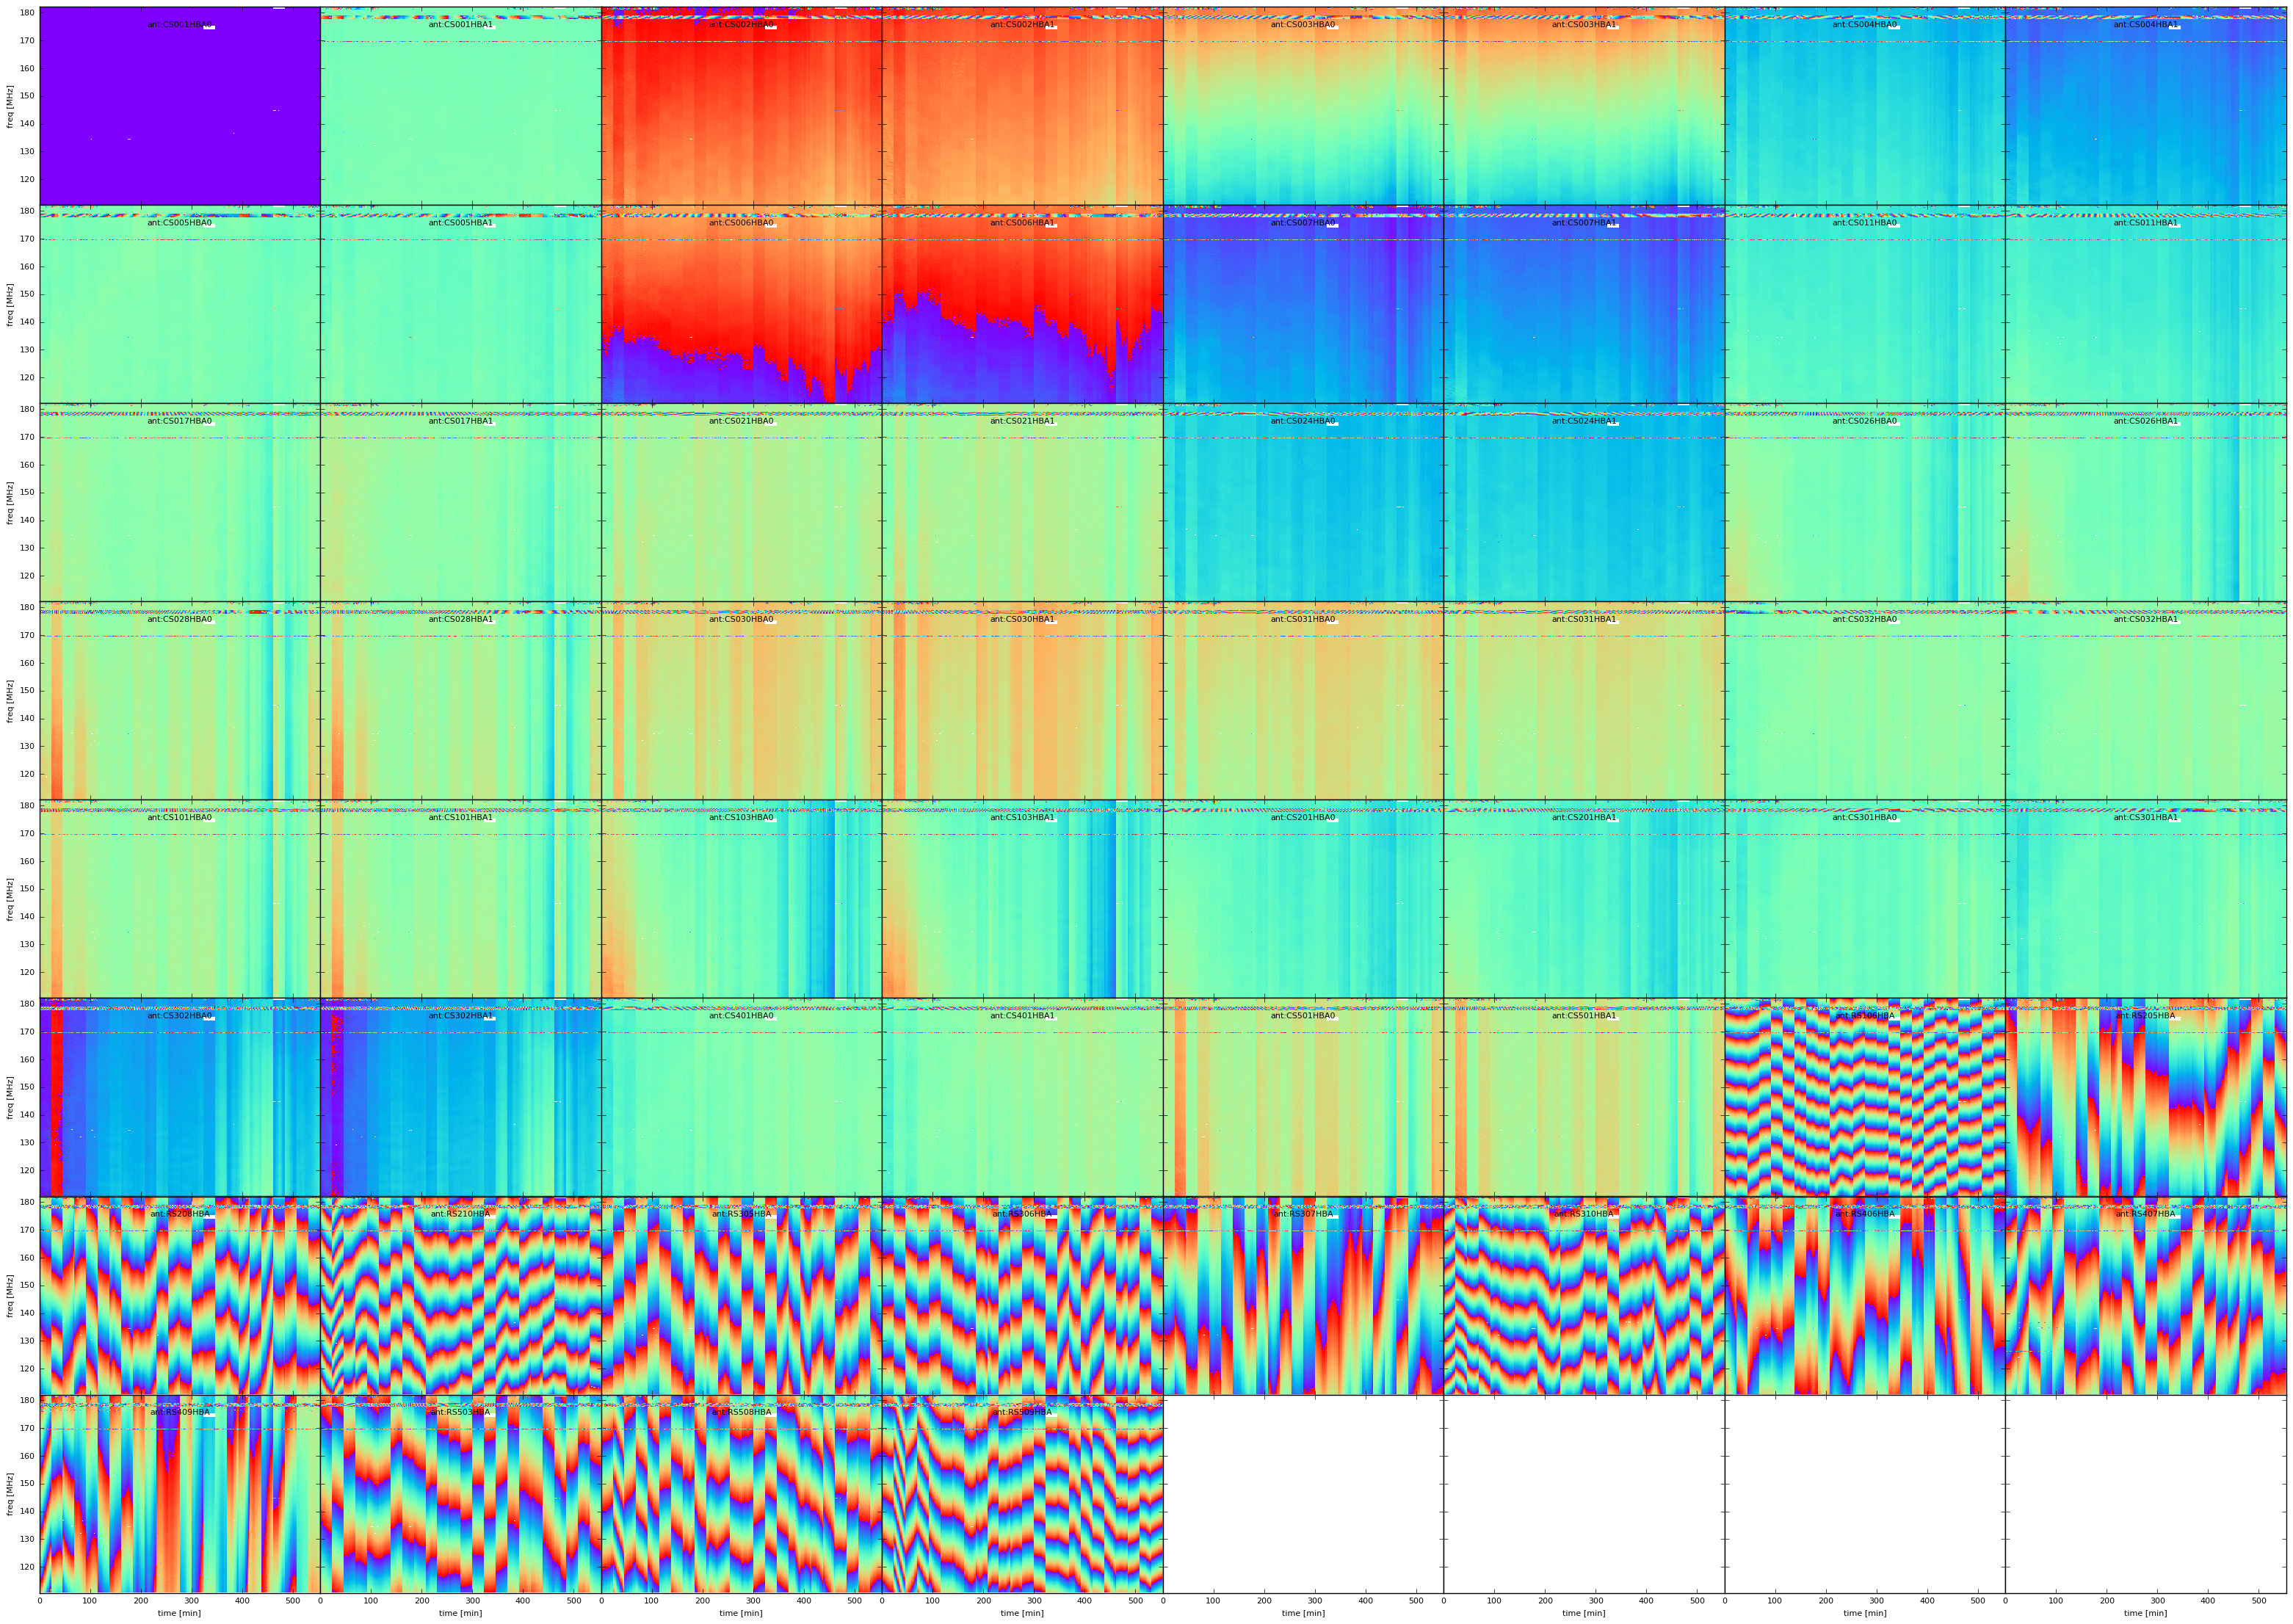
\includegraphics[height = 6cm,width=7.5cm]{cal_phases_polYY_dirpointing.png}
		 &  This plot shows the calibrator solutions in the YY polarisation. The CS001HBA0 station is flagged, and some of the frequencies between 170 to 180~MHz seem to have noisy data. \\
\midrule\addlinespace[1.5ex]
         \includegraphics[height = 6.5cm,width=8.2cm]{matrix_xx.png}
         & This hows the waterfall plots of the amplitude solutions for the single stations. It can be used to see which stations are bad in the first plot.\\
\end{tabular}
\end{table}    
\newpage
\begin{table}[ht] 
\centering        
\begin{tabular}{m{8.5cm}|m{4.5cm} }      % centered columns (3 columns) 
\hline\hline                                      %inserts double horizontal lines 
Diagnostic plots  & Description \\ [0.5ex] % inserts table heading 
\midrule\addlinespace[1.5ex]
         \includegraphics[height = 6cm,width=7.5cm]{dtec_allsols.png}
         & This plot shows the differential Total Electron Content (dTEC). It shows that the data is fine, even though it may noisy.\\
\midrule\addlinespace[1.5ex]
         \includegraphics[height = 6cm,width=7.5cm]{dclock_allsols.png}
         & This plot shows the differential clock values. For all the core stations, the values should lie on 0.\\
\midrule\addlinespace[1.5ex]
		 \includegraphics[height = 6.5cm,width=7.8cm]{phase_xx_yy_offset.png}
		 & This plot gives the median difference of the phase solutions for the X and the Y antennas. For the station calibration, the X and Y dipole phases are not aligned with each other resulting in phase offsets. The blue spikes represent the ones that have been flagged by pre-factor.\\
\end{tabular}
\caption{This table shows the diagnostic plots that are obtained as an output from the Prefactor pipeline. They give an overview of the condition of the data and help us select and flag any data sets that seem bad, and were not previously flagged by the pipeline.}
\label{diagnostic}    
\end{table}


\section{Imaging}
\verb|Common Astronomy Software Application|\footnote{\url{https://casa.nrao.edu/}} was used to make images of the two galaxies. The visibilities of the target facet were used to make the images of both the galaxies. The LOFAR primary beam is much larger than the size of the galaxies, and hence, LOFAR primary beam correction was not done.  
\paragraph{For IC 342}:Three images of varying resolutions were made. The noise of each image was obtained from the rms value of a region around a part of the image with no source. The images were made using the multi-scale clean technique. The outer taper for the image in figure \ref{img1} was 14~arcsec by 9.5~arcsec. or figure \ref{img2}, the outer taper was 22~arcsec by 22~arcsec, and for the image \ref{img3}, the outer taper used was 23~arsec by 24~arcsec.

\begin{figure}[h]
\centering
\includegraphics[scale=0.4]{IC342_images/Image_1.png}
\caption{This is the LOFAR image of IC342 at the central frequency of 146.2~MHz. Bandwidth of the observation was 62.5~MHz. This image has the resolution of 12.48" by 10.26"; PA: -8.10 deg. The contours are at 3, 8, 12, 18, 18, 32 and 44 of 0.3~mJy/beam, which is the noise of the image in a quiet region.}
\label{img1}
\end{figure}

\begin{figure}[h]
\centering
\includegraphics[scale = 0.4]{IC342_images/Image_3.png}
\caption{This image has the resolution of 25.93" by 23.26"; PA: 62.7 deg. The contours are at 3, 8, 12, 18, 18, 32 and 44 of 0.43~mJy/beam.}
\label{img2}
\end{figure}

\begin{figure}[h]
\centering
\includegraphics[scale = 0.4]{IC342_images/Image_5.png}
\caption{This image has the resolution of 38.15" by 34.39"; PA: 23.99 deg. The contours are at 3, 8, 12, 18, 18, 32 and 44 of 0.6~mJy/beam.}
\label{img3}
\end{figure}

\end{document}

